\begin{frame}
  \frametitle{A Search Algorithm}
  \centering
  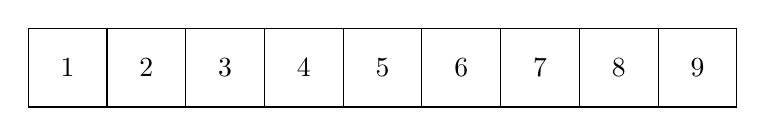
\begin{tikzpicture}
    \draw[draw=black] (0,0) rectangle (1,1) node[pos=0.5] {1};
    \draw[draw=black] (1,0) rectangle (2,1) node[pos=0.5] {2};
    \draw[draw=black] (2,0) rectangle (3,1) node[pos=0.5] {3};
    \draw[draw=black] (3,0) rectangle (4,1) node[pos=0.5] {4};
    \draw[draw=black] (4,0) rectangle (5,1) node[pos=0.5] {5};
    \draw[draw=black] (5,0) rectangle (6,1) node[pos=0.5] {6};
    \draw[draw=black] (6,0) rectangle (7,1) node[pos=0.5] {7};
    \draw[draw=black] (7,0) rectangle (8,1) node[pos=0.5] {8};
    \draw[draw=black] (8,0) rectangle (9,1) node[pos=0.5] {9};
  \end{tikzpicture}
\end{frame}


\begin{frame}
  \frametitle{A Better Search Algorithm}
  \centering
  \begin{tikzpicture}

    \pgfmathtruncatemacro{\asize}{9}
    \pgfmathtruncatemacro{\N}{3}
    \readlist\values{5,7,8}

    \foreach \n in {1,2,...,\N}{
      \onslide<\n>{
        \foreach \i in {1,2,3,...,\asize}{
          \ifnum\i=\values[\n]
            \draw[draw=black] (\i-1,0) rectangle (\i,1) node[pos=0.5] {\i};
          \else
            \draw[draw=white, fill=black] (\i-1,0) rectangle (\i,1);
          \fi
        }
      }
    }
  \end{tikzpicture}
\end{frame}

